Since the beginning of time, early human settlements were eager to explore their environment and surroundings. It did not take long, until the very first humans started getting even further and eventually become explorers. They left marks and started using landmarks to remember pathways and places. This primitive representation of prehistoric places and early history maps can be traced back to 24000-25000 BC\cite{cavedrawings}. Soon after, they started using maps, which revolutionized the way we navigate and the way we travel, - and therefore the field of Cartography was born. During the 19th century, terra incognita \textit{(orig. Latin, ‘unknown land.’)} disappeared from maps, since both the coastlines and the inner parts of the continents had been fully explored. Today, using technology and satellites, Earth is completely mapped\cite{earth-mapped}, yet still not completely explored\cite{earth-explored}. Around 95 percent of our oceans still remains unexplored, considering that they take up 70 percent of the planet's surface\cite{oceandepth}. This is mostly due to extreme conditions and high depths, that humans can not be put up against. As technology advanced and matured, remotely operated underwater vehicles (ROVs) become a popular way of exploring the depths of the oceans, due to their accessibility to places where humans could not possibly go before for a long period of time. In the meantime, interplanetary exploration took off during the mid-20th century with the start of the Cold War between the United States of America and the Soviet Union. This led to many great achievements in the field of rocket science and space exploration, like the first successful interplanetary encounter, where the US Mariner 2 flew by Venus\cite{firstflyby} or when the Soviet Venera 3 made first impact on the surface of Venus\cite{firstimpact}. One of the latest successful programs is the Mars rover CURIOSITY\cite{curiosity}, which landed and still is making progress in exploring and sending back scientific data of the planet Mars. Exploring planets for future-settlements and first-contact is very important in order to quench out human curiosity but also for advancing the different fields in science and technology.

\clearpage

\begin{figure}[!h]
	\centering
	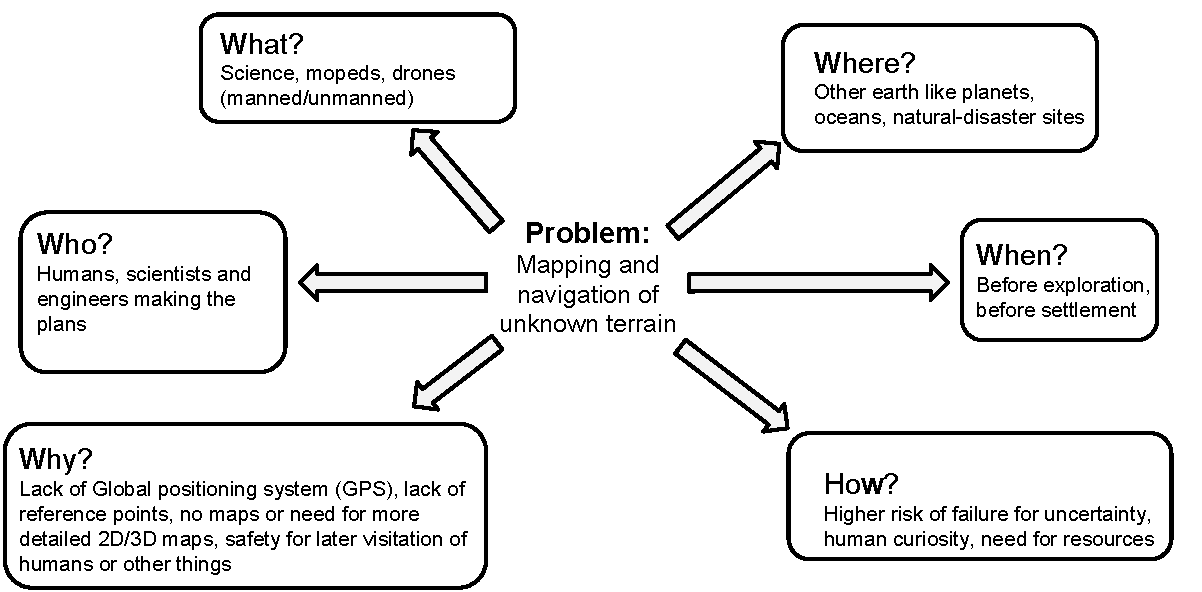
\includegraphics[scale=.7]{images/wdiagram2.pdf}
	\caption{W-diagram}
	\label{fig:wdiagram}
\end{figure}

\subsection{When is this actually a problem?}
Mapping unknown terrains becomes a problem when new planets are discovered and mapping of the surface and its atmosphere is necessary for further exploration and investigation of the planet. Scientists use the so-called Earth Similarity Index (ESI) for mapping extrasolar planets (also called exoplanets) for potentially habitable places in the Universe\cite{exoplanets}\cite{esi}. The ESI index implies many factors, like surface temperature and other Earth-like properties. 

Another scenario is underwater exploration, where trained divers are unable to explore and map the underwater terrain due to its depth and dangerous circumstances. In these cases robots and submarines, that are either autonomously or remotely controlled, can take up the task of mapping the bottom of the ocean. It is also much faster and more reliable than sending down people to do the same task.

Besides exploration, the task of mapping unknown terrains is used in the event of a hostage situation or natural disaster as well, where people cannot enter a specific area without it being mapped upfront for various factors, like radiation leakage or armed terrorists. One example would be the Fukushima Nuclear Plant catastrophe in Fukushima, Japan on March, 2011. After the leakage in the reactor, rescue forces and scientist used autonomous drones to map the inside of the factory\cite{fukushima}, which was put under quarantine for high levels of radiation and therefore no person was allowed inside of the building without proper precautions. Drones and autonomous robots are perfect for scenarios like this.

\clearpage

\subsection{Where does this problem actually occur?}
An unknown terrain can be defined as a terrain where no mapping has been done before.

The bottom of the ocean is mostly sand, mud, and water\cite{bottom-composition}. This makes it difficult to navigate with a rover, but relatively simple with a submarine. In water, sensors that use sound, need to be calibrated to work with the correct pressure of the surroundings, which varies with the depth of the water. If the water is murky, light-based sensors may also not work, depending on the wavelength of the light they use. Light also refracts in water depending on the water density. It is possible to remote-control vehicles on the bottom of the ocean. %TODO: Based on what? Feels incomplete.

Other planets can be much more complicated to navigate. The consistency of their atmosphere and terrain may be not completely known. This means that there is a higher chance of a rover being stuck on loose terrain, falling down sheer faces, and so on. It may also be the case that the planet has no atmosphere, so a drone would not be able to hover. One of the biggest issues with extraplanetary exploration is input lag. Other planets are very far away, which means that signals travelling to these distant places can take several minutes at least and years at most to reach from planet Earth. Thus automation is better suited for this task. Other planets also share the issues that the bottom of the ocean has, namely that sensors need to be calibrated to the different atmospheric levels and other characteristics of the planet.

Disaster scenarios can also be classified as unknown terrain. This means that the terrain might be loose or difficult to navigate, so a drone might be best suited for it. In most cases, disaster scenarios happen in locations where a vehicle can be controlled manually.

\subsection{How is it a problem?}

To answer the question of how this is a problem, we have to look into some possible scenarios discussed above. Exploration of unknown terrain and environments has been practised for many years now. It originates from the human curiosity and the spirit to explore and gather information about our surroundings, as discussed previously.

When dealing with unknown environments, the word \textit{'unknown'} does not strictly refer to the environment itself but the persons state of knowledge about the physics and composition of the given environment. In a known environment, outcomes from every action can more or less be calculated or estimated. Where as in an unknown environment, it is a matter of investigation and figuring out what works and what does not. In the unknown environment it is important to gain knowledge of how everything works, so that in the future it is possible for an individual to take the best possible choices and decisions in the said environment\cite{aiint}.
Even though most of the land has been explored and is being used for its vast amount of resources, the time will come where planetary and ocean exploration becomes a key factor for our technological advancements and our own resources on planet Earth. Ocean exploration is important because it provides data from deep-sea areas, which in turn will reduce the amount of unknown environments left on our planet.
Gathering data and intelligence from the ocean also helps with managing the resources that are available in the deep-sea areas, so that future generations can benefit from them. The ocean also provides information about future environmental conditions and can help predict earthquakes and tsunamis. Investigating the deep-sea also reveals new ecosystems and possible sources for medication, food and energy, which are all vital for scientific advancements or survival on Earth\cite{oceanexplo}.

Humans have always had never-ending interest and the need to push science and technology over its limits, and a desire to achieve something even further than what is possible. The many challenges humans have faced so far, has led to many benefits for our society since its creation. Space exploration helps to further our understanding about the history of our universe and solar system\cite{whyweexplo}.

\subsection{To whom and what is this a problem?}
Unknown terrains and environments pose a big issue for scientists and engineers who want to explore these areas. Designing vehicles and devices for the deep-sea ocean or planetary exploration is impossible without any background information on what environmental factors they will be dealing with or encountering during the set mission. Exploration is essential when, in the future, new resources are needed for scientific and technological advancements, that is currently out of our reach.

In the long run, humans in general will be affected by the lack of exploration. Alternative resources and habitable areas for expansion will be necessary in the future, when Earth's natural resource-deposits become depleted and no habitable places left. 

Scientists are heavily hindered by society, because it is becoming too focused on risks. Only 5 percent of the ocean has been explored so far, which leaves a large amount of areas untouched and unmapped. Being concerned about taking risks is what will put the future development and science in jeopardy\cite{risksandexplo}. 

\subsection{Why is this a problem?}
The reason why there is a need to explore other unknown terrains is to help better understand everything around us and to be able to go to other planets. 
If the trips are well planned and a sufficient 3D map of the terrain is generated, it is possible to more optimally plan-ahead for the next mission or to determine if the environment is worth exploring further or visiting once again. 

The problems with navigating a robot in an unknown terrain is the lack of reference points that are needed to make a 2D or 3D map and reference points for the robot itself to being able to navigate and find its way around. This creates two challenges: one, is for the robot to be able to navigate through a completely unknown terrain and secondly, to make sense of it and come up with reference points and data that can be converted into a map.

If a robot is successful at navigating unknown terrains and gathering data, it can be turned into a detailed map, where the next mission can rely on that information and have a easier way to navigate and possibly a more successful mission. 

On Earth, we have the GPS (global positioning system), which is a space-based satellite navigation system placed above Earth\cite{gpsgeneral}. Putting up a system like that on another planet would cost a lot of resources and is not beneficial for first-time exploration missions. GPS also does not penetrate water\cite{underwatergps}.
